%!TEX TS-program = xelatex
%!TEX encoding = UTF-8 Unicode

\documentclass[12pt]{article}
\usepackage{geometry}                % See geometry.pdf to learn the layout options. There are lots.
\geometry{a4paper,top=2cm}
\usepackage[parfill]{parskip}    % Activate to begin paragraphs with an empty line rather than an indent
\usepackage{graphicx}
\usepackage{amsmath}
\usepackage{amssymb}
\usepackage{mathtools}
\usepackage{physics}
\newcommand{\be}{\begin{equation}}
\newcommand{\ee}{\end{equation}}
\usepackage[thicklines]{cancel}
\usepackage{url}
\usepackage{booktabs}
\usepackage{csquotes}
\usepackage{qcircuit}
\usepackage{circledsteps}
\usepackage{nicefrac}
\usepackage{fontspec,xltxtra,xunicode}
\usepackage{xcolor}
\defaultfontfeatures{Mapping=tex-text}

\newcommand{\polv}{\ensuremath{\updownarrow}}
\newcommand{\polh}{\ensuremath{\leftrightarrow}}
\newcommand{\poldr}{\rotatebox[origin=c]{45}{\ensuremath{\leftrightarrow}}}
\newcommand{\poldl}{\rotatebox[origin=c]{-45}{\ensuremath{\leftrightarrow}}}
\newcommand{\bigzero}{\mbox{\normalfont\Large\bfseries 0}}

\title{Advanced Quantum Mechanics\\Class 22 (a)}
%\author{The Author}
\date{October 25, 2022}                                           % Activate to display a given date or no date

\setcounter{section}{6}
\setcounter{subsection}{7}
\setcounter{equation}{85}

\begin{document}
\maketitle

%%% 01 OKAY

\subsection{Parity}

Parity reverses the sign of the coordinates:
\be
P: \vec{r} \to \vec{r}^\prime = P\vec{r} = -\vec{r}
\ee
$P$ can be viewed as:\\
 -- Reflection with respect to a plane.\\
 \phantom{ -- Reflection with}+\\
 -- Rotation by $\pi$ about an axis $\perp$ to this plane.\\
Take as example the $xOy$ plane and $M$ the reflexion 
with respect to this plane, and $R_z(\pi)$ the rotation
about $O_z$:
\be
\vec{r} = \begin{pmatrix}x\\y\\z\end{pmatrix}
\stackrel{M}{\longrightarrow} \begin{pmatrix}x\\y\\-z\end{pmatrix}
\stackrel{R_z(\pi)}{\longrightarrow} \begin{pmatrix}-x\\-y\\-z\end{pmatrix}
\ee
Rotation invariance is valid in general
$\Rightarrow$
then, the mirror image of a physics experiment
must appear as being physically possible.

\emph{Polar vectors:}
\be
\vec{r}\to-\vec{r}, \quad \vec{p}\to-\vec{p}, \quad \vec{E}\to-\vec{E}
\ee
\emph{Axial vectors:}
\be
\vec{J} = \vec{r} \times \vec{p} \to +\vec{J}, \quad \vec{B} = \vec{\nabla} \times \vec{A} \to \vec{B}
\ee
(remember, $\vec{E} = - \frac{\partial \vec{A}}{\partial t}$).

%%% 02 OKAY

Parity is conserved in strong and electromagnetic (e.m.)
interactions, but \emph{is not} conserved by the weak interaction
$\Rightarrow$ C.S.~Wu (1956).

\begin{displayquote}
Decay of ${ }^{60} \mathrm{Co}$ : decays to ${ }^{60} \mathrm{Ni}^{*}$, one of the neutrons
in ${ }^{60} \mathrm{Co}$ decays to $p+e^{-}+\bar{\nu}_{e}$ (weak decay) and the
${ }^{60} \mathrm{Ni}^{*}$ decays rapidly to ${ }^{60} \mathrm{Ni}+2 \gamma$ (e.m. decay).

Experiment: used polarized nuclei; polarization
achieved with high external magnetic fields.
If electrons would have no preference direction of
decay relative to the direction of the nuclear spin,
parity would be conserved
$\Rightarrow$
but C.S. Wu \textit{et al.} found that
the electrons were emitted preferentially
in a direction opposite of the
nuclear spin.
\end{displayquote}

In real space $P$ together with the identity:
\be
P\vec{r} = - \vec{r},\quad I\vec{r} = \vec{r}
\ee
form an Abelian group. How is the action of this
%%% 03 OKAY
group in Hilbert space $H$?
\begin{itemize}
\item Let $\hat{\Pi}$ represent the parity transformation in $H$.
%
\item Since two successive parity transformations
are equivalent to the identity, the eigenvalues
of $\hat{\Pi}$ are $\pm1$.
%
\item If parity is conserved, $\hat{\Pi}$ commutes with
the Hamiltonian
\be
[\hat{\Pi},\hat{H}] = 0
\ee
hence it is possible to find a set of eigenvectors
$\ket{\varphi_\pm}$ common to $\hat{H}$ and $\hat{\Pi}$:
\be
\hat{\Pi}\ket{\varphi_\pm} = \pm\ket{\varphi_\pm},\quad
\hat{H}\ket{\varphi_\pm} = E_\pm \ket{\varphi_\pm}
\ee
%
\item In a coordinate representation:
\be
\bra{\vec{r}}\ket{\varphi_\pm} = \varphi_\pm(\vec{r})
\ee
therefore
\be
\hat{\Pi} \varphi_\pm(\vec{r}) =  \varphi_\pm(-\vec{r}) = \pm \varphi_\pm(\vec{r})
\ee
\[
\begin{aligned}
\varphi_+(\vec{r}):& \text{ even function; positive parity}\\
\varphi_-(\vec{r}):& \text{ odd function; positive parity}\\
\end{aligned}
\]
%%% 04 OKAY
\item therefore, the group $\{P,I\}$ can be associated
with the group of two elements $\{+1,-1\}$, the
group $Z_2$.
\end{itemize}

Since elements $+1$ and $-1$ cannot be connected
to each other continuously, is $\hat{\Pi}$ a unitary or
an antiunitary operator? $\Rightarrow$
Let $\ket{\varphi}$ and $\ket{\chi}$ be arbitrary vectors of $H$,
and also consider $\ket{c\varphi} = c\ket{\varphi}$, $\ket{c\chi} = c\ket{\chi}$

\fbox{\begin{minipage}{\textwidth}
Let's use the ordered pair notation for inner products here, 
and remember that the inner product is 
antilinear in the \emph{first} entry,
while being linear in the in the \emph{second} entry.
\[
\begin{aligned}
\bra{\varphi}\ket{c\chi} &\equiv (\varphi,c\chi) = c  (\varphi,\chi)\\
\bra{c\varphi}\ket{\chi} &\equiv (c\varphi,\chi) = c^*(\varphi,\chi)
\end{aligned}
\]
\end{minipage}
}

If parity is a symmetry:
\be
|(\hat{\Pi}\chi,\hat{\Pi}\varphi)| = |(\chi,\varphi)|
\ee
In $H$, we also have:
\be
\begin{aligned}
\hat{\vec{R}} \rightarrow \hat{\vec{R}}^\prime = \hat{\Pi}^{-1} \hat{\vec{R}}\,\hat{\Pi} = -\hat{\vec{R}} &\Rightarrow \hat{\Pi}\hat{\vec{R}} = - \hat{\vec{R}}\hat{\Pi}\\
\hat{\vec{P}} \rightarrow \hat{\vec{P}}^\prime = \hat{\Pi}^{-1} \hat{\vec{P}}\,\hat{\Pi} = -\hat{\vec{P}}
&\Rightarrow \hat{\Pi}\hat{\vec{P}} = - \hat{\vec{P}}\hat{\Pi}
\end{aligned}
\ee
and (note reverse order of $\hat{\Pi}$ and $\hat{\Pi}^{-1}$)
\be
\hat{\Pi} [\hat{X}_i,\hat{P}_j] \hat{\Pi}^{-1} = [\hat{X}_i,\hat{P}_j] = i \hbar \delta_{ij}
\ee
On the other hand:
\begin{enumerate}
\item 
\be
\begin{gathered}
\left(\hat{\Pi} \chi, \hat{\Pi}\left[\hat{X}_{i}, \hat{P}_{j}\right] \varphi\right)=\left(\hat{\Pi} \chi, \hat{\Pi}\left[\hat{X}_{i}, \hat{P}_{j}\right] \hat{\Pi}^{-1} \hat{\Pi}\varphi\right)\\
=\left(\hat{\Pi} \chi, i \hbar \delta_{i j} \hat{\Pi} \varphi\right)=i \hbar \delta_{i j}(\hat{\Pi} \chi, \hat{\Pi} \varphi)
\end{gathered}
\label{eq:g98}
\ee
and
%%% 05 OKAY
\item
\be
\left(\hat{\Pi} \chi, \hat{\Pi}\left[\hat{X}_{i}, \hat{P}_{j}\right] \varphi\right) = 
\left(\hat{\Pi} \chi, \hat{\Pi} i \hbar \delta_{i j} \varphi\right)
\label{eq:g99}
\ee
\end{enumerate}
Eqs.~\eqref{eq:g98} and \eqref{eq:g99} are compatible if and only if
$\hat{\Pi}$ is unitary, since
for a unitary operator $\hat{U}$
\be
(\hat{U}\chi,\hat{U}i\varphi) = (\chi,i\varphi) = i(\chi,\varphi)
\ee
 while for an antiunitary $\hat{U}$
\be
(\hat{U}\chi,\hat{U}i\varphi) = (i\varphi,\chi) = (\chi,i\varphi)^* = -i(\varphi,\chi)
\ee
 

\subsection{Time reversal}

Let us first examine this issue in \emph{classical
mechanics}, for a situation of time-independent
forces:
\begin{itemize}
\item let $\vec{r}\left(t_{0}\right)$ and $\vec{p}\left(t_{0}\right)$ be the position and
momentum of a particle at the time instant $t_0$
\item after a time interval $t$, the particle is found
at $\vec{r}\left(t_{0}+t\right)$ with a momentum $\vec{p}\left(t_{0}+t\right)$
%%% 06
\item let us suppose that at this instant, $t_0+t$,
another particle, identical to the previous one,
starts its movement with initial conditions
$\vec{r}\left(t_{0}+t\right)$, $-\vec{p}\left(t_{0}+t\right)$
%
\item if after another time interval $t$ this second
particle is found at position $\vec{r}\left(t_{0}\right)$ and
with momentum $-\vec{p}\left(t_{0}\right)$
\end{itemize}
$\Rightarrow$ then, the \emph{dynamics} that governs
the movement is said to be
\emph{invariant under time reversal}.

\begin{figure}[htbp]
\centering
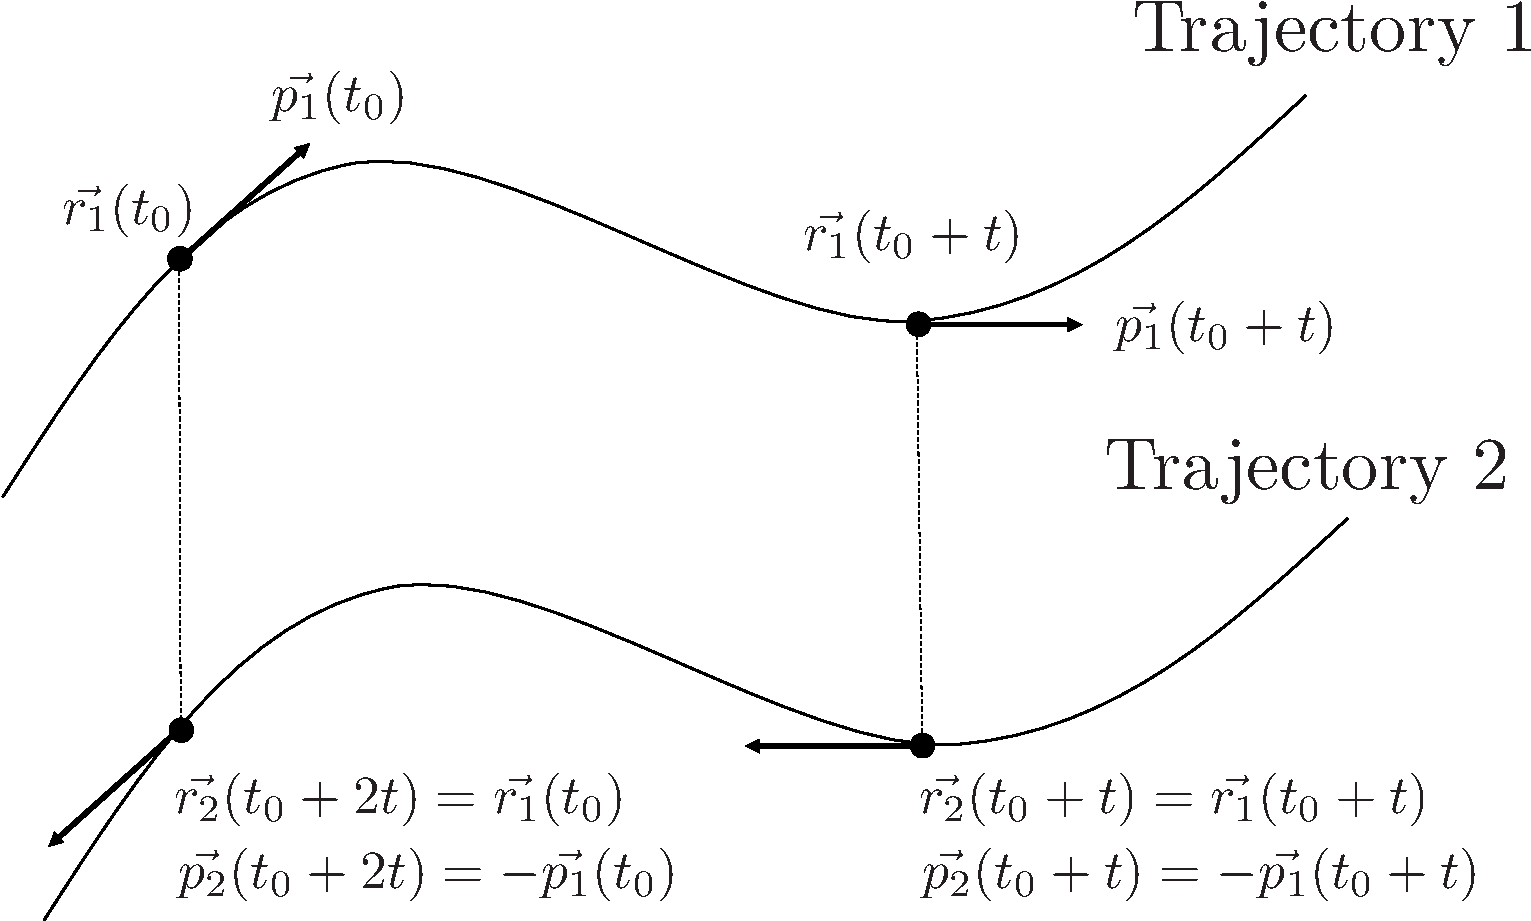
\includegraphics[width=0.75\textwidth]{Figures/TimeReversal1-crop.pdf}
\end{figure}

Classical equations of motion are invariant if for
any trajectory 1 there corresponds another
%%% 07 OKAY
trajectory 2, identical to the first one with
reversed momentum.

\begin{minipage}{0.5\textwidth}%
%\vspace{12em}\hspace{1ex}
\centering
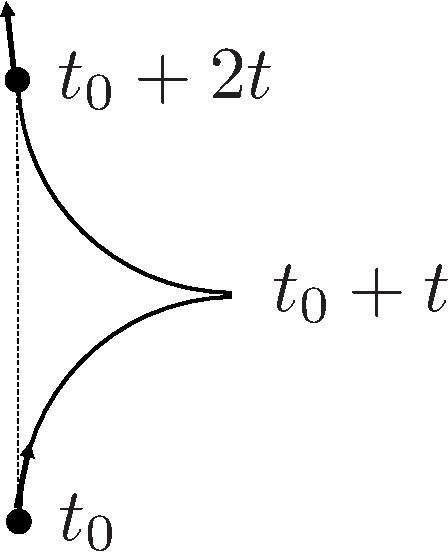
\includegraphics[width=0.4\textwidth]{Figures/TimeReversal2-crop.pdf}
\end{minipage}%
\begin{minipage}{0.5\textwidth}%
Charged particle in the presence of a 
magnetic field $\to$ \emph{NOT} invariant under
time reversal.
\end{minipage}%

\emph{Quantum mechanics}:\\
Let $\hat{\Theta}$ denote the operator that implements time
reversal in $H$:
\be
\begin{aligned}
\hat{\Theta}\hat{\vec{R}}\hat{\Theta}^{-1} &\equiv \hat{\vec{R}}_t = \hat{\vec{R}}\\
\hat{\Theta}\hat{\vec{P}}\hat{\Theta}^{-1} &=      \hat{\vec{P}}_t = -\hat{\vec{P}}\\
\hat{\Theta}\hat{\vec{J}}\hat{\Theta}^{-1} &=  	   \hat{\vec{J}}_t = -\hat{\vec{J}}
\end{aligned}
\ee
where the index $t$ means time reversal. Consider the matrix element of $[\hat{X}_i,\hat{P}_j] = i\hbar\delta_{ij}$:
\begin{enumerate}
\item 
\be
\begin{aligned}
\left(\hat{\Theta}\chi,\hat{\Theta}[\hat{X}_i,\hat{P}_j]\psi\right)
&=\left(\hat{\Theta}\chi,\hat{\Theta}i\hbar\delta_{ij}\psi\right)\\
&=\hbar\delta_{ij}\left(\hat{\Theta}\chi,\hat{\Theta}i\psi\right)
\end{aligned}
\ee
\item
\be
\begin{aligned}
\left(\hat{\Theta}\chi,\hat{\Theta}[\hat{X}_i,\hat{P}_j]\hat{\Theta}^{-1}\hat{\Theta}\psi\right)
&=\left(\hat{\Theta}\chi,-[\hat{X}_i,\hat{P}_j]\hat{\Theta}\psi\right)\\
&=\hbar\delta_{ij}(\hat{\Theta}\chi,-i\hat{\Theta}\psi)
\end{aligned}
\ee
%% 08 OKAY
$\Rightarrow$ compatible if $\hat{\Theta}i = -i\hat{\Theta}$ $\to$ $\hat{\Theta}$ is \emph{antilinear}.
\end{enumerate}

Another way of getting that $\hat{\Theta}$ is antilinear:
\begin{itemize}
\item let $\ket{\varphi(t)}$ be the state at time $t$ and $\ket{\varphi} = \ket{\varphi(t=0)}$:
\be
\ket{\varphi(t)} = \ket{e^{-i/\hbar\hat{H}t}\varphi(0)} = e^{-i/\hbar\hat{H}t\ket{\varphi}}
\ee
%
\item invariance under time reversal implies that the
state transformed from $|\varphi(-t)\rangle$ by time reversal,
i.e. $|\hat{\Theta} \varphi(-t)\rangle$, coincides with the state obtained
by the time evolution of $|\hat{\Theta} \varphi(0)\rangle$:
\[
\ket{\hat{\Theta} \varphi(-t)} = \ket{e^{-i/\hbar\hat{H}t}\hat{\Theta}\varphi(0)}
\]
but $\varphi(-t)$ is $e^{-i/\hbar\hat{H}(-t)}\varphi(0)$, so
\[
\ket{\hat{\Theta} e^{-i/\hbar\hat{H}(-t)}\varphi} = \ket{e^{-i/\hbar\hat{H}t}\hat{\Theta}\varphi}
\]
hence
\be
\hat{\Theta}e^{i/\hbar\hat{H}t} = e^{-i/\hbar\hat{H}t}\hat{\Theta}
\label{eq:g106}
\ee
\end{itemize}
If $\hat{\Theta}$ \emph{were} unitary, Eq.~\eqref{eq:g106} would imply
\be
\hat{\Theta}\hat{H} = -\hat{H}\hat{\Theta}
\ee
so
\[
\hat{H}\varphi_E = E\varphi_E \to \hat{H}\hat{\Theta}\varphi_E 
= -\hat{\Theta}\hat{H}\varphi_E = -E\hat{\Theta}\varphi_E
\]
$E$ belonging to an energy spectrum 
from \textit{e.g.} 0 to infinity.
So the second equality 
\emph{would} imply an instability, 
as the energy would not be
bounded from below.

%%% 09 OKAY

Nothing of this happens if $\hat{\Theta}$ is antiunitary:
\[
[\hat{H},\hat{\Theta}] = 0 \text{ as } 
\hat{\Theta}i\hat{H} = -i\hat{\Theta}\hat{H} = -i\hat{H}\hat{\Theta}
\]
\emph{BUT} $\hat{\Theta}$ \emph{does not} lead to a conserved quantity,
since
\be
\frac{d}{d t}\langle\hat{A}\rangle_{\varphi}=\frac{i}{\hbar}\langle[\hat{H}, \hat{\Theta}]\rangle
\ee
applies to an $\hat{A} = \hat{A}^{\dagger}$.
$\hat{\Theta}$ is a good symmetry for all fundamental interactions,
but its breaking has been observed in $K^0$-$\overline{K}^0$ meson
system (and also in B mesons) $\leftarrow$ actually CP violation.

Double time reversal $\sim I$: $\hat{\Theta}^2\varphi\sim\varphi$ up to a phase:
\begin{itemize}
\item $\varphi$,$\psi$ two arbitrary states
\item $\hat{\Theta}^2 = cI$, $[(\hat{U}\varphi,\hat{U}\chi) = (\chi,\varphi)]$ since it is antiunitary.
\be
\begin{aligned}
(\hat{\Theta} \varphi, \psi) 
&=\left(\hat{\Theta} \psi, \hat{\Theta}^{2} \varphi\right)=c(\hat{\Theta} \psi, \varphi)=c\left(\hat{\Theta} \varphi, \hat{\Theta}^{2} \psi\right) \\ 
&=c^{2}(\hat{\Theta} \varphi, \psi) \Rightarrow c^{2}=1 \rightarrow c=\pm 1
\end{aligned}
\label{eq:g109}
\ee
\end{itemize}

In general, the action of $\hat{\Theta}$ on state vectors and
operators can be made in two steps: complex conjugation
followed by a unitary transformation.
%%% 10 OKAY
Let us see how this comes about.

Let $\{\ket{n}\}$ (discrete or continuous) be an orthonormal basis in $H$, and
$\{\ket{n_t}\} = \{\ket*{\hat{\Theta}n}\}$ The two bases are related by
a \emph{unitary} transformation:
\be
\hat{U}_{t}=\sum_{n}|n_{t}\rangle\langle n|=\sum_{n}| \hat{\Theta} n\rangle\langle n|
\label{eq:g110}
\ee
therefore
\be
\hat{U}_{t}|n\rangle=\sum_{m}\left|m_{t}\right\rangle\langle m | n\rangle=\left|n_{t}\right\rangle
\ee
(the sum is to be substituted by an integral in the case of a continuous basis).

\clearpage
\par\noindent\rule{\textwidth}{1pt}
Before proceeding, let us prove that $\hat{U}_t$ is really unitary.
Use Eq.~\eqref{eq:g110} for the expression of $\hat{U}_t$:
\be
\begin{aligned}
\bra{\varphi}\hat{U}_t\hat{U}_t^\dagger\ket{\varphi}
& = \bra{\varphi} \sum_n \ket{\hat{\Theta}n}\bra{n} \sum_m \ket{m}\bra{\hat{\Theta}m} \ket{\varphi}
 = \sum_{n,m} \bra{\varphi} \ket{\hat{\Theta}n} \bra{n}\ket{m} \bra{\hat{\Theta}m} \ket{\varphi}\\
& = \sum_{n} \bra{\varphi} \ket{\hat{\Theta}n} \bra{\hat{\Theta}n} \ket{\varphi}
 = \sum_{n} \bra{\hat{\Theta}^2 n} \ket{\hat{\Theta}\varphi} \bra{\hat{\Theta}\varphi} \ket{\hat{\Theta}^2 n},\text{ use Eq.~\eqref{eq:g109}} \\
& = \sum_{n} \bra{n} \ket{\hat{\Theta}\varphi} \bra{\hat{\Theta}\varphi} \ket{n}
 = \sum_{n} \bra{\hat{\Theta}\varphi} \ket{n}\bra{n} \ket{\hat{\Theta}\varphi}\\
& = \bra{\hat{\Theta}\varphi} \ket{\hat{\Theta}\varphi} = \bra{\varphi}\ket{\varphi}
\end{aligned}
\ee
Since $\ket{\varphi}$ is arbitrary:
\be
\hat{U}_t\hat{U}_t^\dagger = I = \hat{U}_t^\dagger\hat{U}_t
\ee
where the second equality is left as an exercise.

\par\noindent\rule{\textwidth}{1pt}
%%% 11 OKAY

Coming back to the main discussion, since $\hat{\Theta}$ is antiunitary:
\be
\begin{aligned}
|\hat{\Theta} \varphi\rangle 
&=\hat{\Theta}|\varphi\rangle=|\varphi_{t}\rangle \\ 
&=\hat{\Theta} \sum_{n}|n\rangle\langle n | \varphi\rangle=\sum_{n}\left|n_{t}\right\rangle\langle n | \varphi\rangle^{*} \\
&=\sum_{n} \hat{U}_{t}|n\rangle\langle n | \varphi\rangle^{*} =\hat{U}_{t} \sum_{n}|n\rangle\langle n | \varphi\rangle^{*} \\ 
&=\hat{U}_{t} \sum_{n}\langle n | \varphi\rangle^{*}|n\rangle
\end{aligned}
\label{eq:g114}
\ee
%
%.    \hat{\Theta}
%
Action of $\hat{\Theta}$ on $\ket{\varphi}$ can be written equivalently as
\be
\hat{\Theta} = \hat{U}_t \hat{\Theta}_0,\,\hat{\Theta}_0:\text{ complex conjugation}
\ee
\emph{Note that:} $\hat{U}_t$ depends on the basis; \textit{e.g.} $\hat{U} = \mathbf{1}$ in
coordinate repres., in momentum repr. $\hat{U}: \ket{\vec{p}} \to \ket{-\vec{p}}$.
We will now want to build this unitary transformation $\hat{U}_t$.

%%% 12 OKAY

Sometimes one needs to relate matrix elements of
an operator between time-reversed states, \textit{e.g.} in
scattering processes, where one often needs to relate
an $i \rightarrow f$ process to its time-reversed motion $f \rightarrow i$.

Let $\hat{A}$ be an arbitrary linear operator in $H$ and
$|\varphi\rangle$ an arbitrary vector in $H$. From Eq.~\eqref{eq:g114},
one has:
\be
\hat{\Theta} \hat{A} \ket{\varphi}=
\begin{cases}
\begin{aligned}
\hat{\Theta}\!\left(\sum_n\op{n}\hat{A}\ket{\varphi}\right) 
&= \sum_n \op{n_t}{n}\hat{A}\ket{\varphi}^*
= \sum_n \op{n_t}{\varphi}\hat{A}^{\dagger}\ket{n}\\
\text{also: }\hat{\Theta}\hat{A}\hat{\Theta}^{-1}\hat{\Theta}\ket{\varphi} 
&= \sum_n \op{n_t}{n}\hat{A}\hat{\Theta}^{-1}\ket{\varphi_t}^*
\end{aligned}
\end{cases}
\ee
whence we identify
\[
\bra{\varphi}\hat{A}^{\dagger}\ket{n} = \bra{n}\hat{A}\hat{\Theta}^{-1}\ket{\varphi_t}^*
\]
%
Let $\ket{\psi}$ be another arbitrary state in $H$. We write 
$\hat{A}_t = \hat{\Theta}\hat{A}\hat{\Theta}^{-1}$
and
$\hat{\Theta}\ket{\psi} = \ket{\psi_t}$.
Then:
\be
\begin{gathered}
\bra{\psi_t}\hat{A}_t\ket{\varphi_t} =
\bra{\psi_t}\hat{\Theta}\hat{A}\hat{\Theta}^{-1}\ket{\varphi_t}\\
 = \bra{\psi_t}\hat{\Theta}\left(
\sum_n\op{n}\hat{A}\hat{\Theta}^{-1}\ket{\varphi_t}
\right)
 = \bra{\psi_t}\left(
\sum_n\ket{n_t}(\bra{n}\hat{A}\hat{\Theta}^{-1}\ket{\varphi_t})^*
\right)\\
=\sum_n \bra{\psi_t}\ket{n_t} \bra{\varphi}\hat{A}^{\dagger}\ket{n}
=\sum_n \bra{n}\ket{\psi} \bra{\varphi}\hat{A}^{\dagger}\ket{n}\\
=\sum_n \bra{\varphi}\hat{A}^{\dagger} \ket{n}\!\!\bra{n}\ket{\psi}
= \bra{\varphi}\hat{A}^{\dagger}\ket{\psi}
\end{gathered}
\ee
When $\hat{A}^{\dagger} = \hat{A}$ and time-reversal invariant:
\be
\bra{\psi_t}\hat{\Theta}\hat{A}\hat{\Theta}^{-1}\ket{\varphi_t} = 
\bra{\psi_t}\hat{A}\ket{\varphi_t} =
\bra{\varphi}\hat{A}\ket{\psi}
\ee
so
\[
(\varphi_t \to \psi_t) \leftarrow \text{ time reversal }\rightarrow (\psi \to \varphi).
\]














\end{document}




















